%
% section 2.4.2
%

\setcounter{subsection}{1}
\subsection{Διευθύνσεις Ελέγχου Πρόσβασης στο Μέσο (MAC) -- Δομή Πλαισίου Ethernet}

\begin{figure}[!ht]
  \centering
  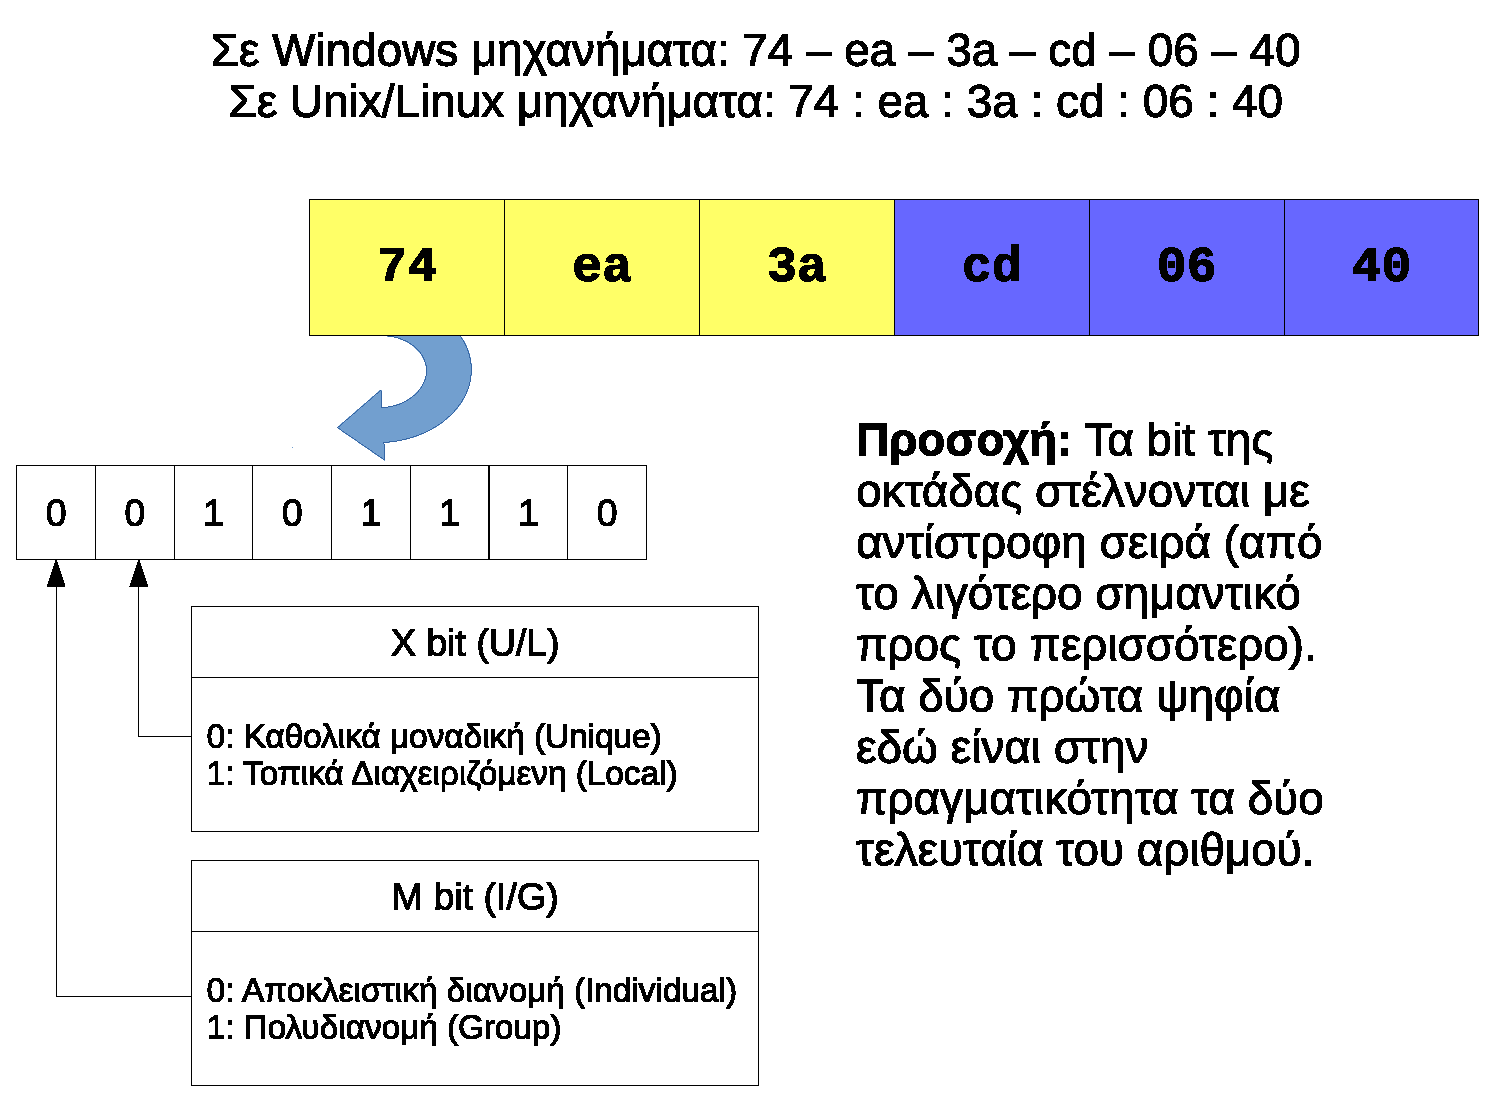
\includegraphics[width=0.95\textwidth]{images/chapter2/2-3}
  \caption {\textsl{Δομή Διεύθυνσης MAC στο Ethernet}}
  \label{2-3}
\end{figure}

Όπως ξέρουμε ήδη, σε ένα δίκτυο Ethernet κάθε κόμβος έχει μια \emph{φυσική διεύθυνση} (MAC address) ή \emph{διεύθυνση υλικού} (Hardware Address) με την οποία αναγνωρίζεται με μοναδικό τρόπο σε όλο το δίκτυο. Η διεύθυνση αυτή αναφέρεται και ως διεύθυνσης προσπέλασης στο μέσο (Media Access Control, MAC) και είναι ένας δυαδικός αριθμός μεγέθους 48 bit ή έξι οκτάδων (bytes).
Γράφεται ως δεκαεξαδικός αριθμός χωρισμένος ανά οκτάδα με παύλες (όταν τον βλέπουμε στα Windows) ή με άνω-κάτω τελείες σε συστήματα Unix/Linux. Ένα παράδειγμα είναι η διεύθυνση:

\begin{center}
74:ea:3a:cd:06:40
\end{center}

(Σημείωση: τα γράμματα μπορεί να είναι μικρά ή κεφαλαία -- δεν υπάρχει διαφορά)

\begin{inthebox}
\textbf{Γιατί τόσο πολύ δεκαεξαδικό στους υπολογιστές;}

Η επιλογή του δεκαεξαδικού συστήματος για τις φυσικές διευθύνσεις (και όχι μόνο) στην αρχή φαίνεται κάπως παράξενη. Εξάλλου οι άνθρωποι έχουμε συνηθίσει στο δεκαδικό και οι υπολογιστές λειτουργούν εσωτερικά στο δυαδικό. Για ποιο λόγο να εισάγουμε ακόμα ένα αριθμητικό σύστημα στην πληροφορική;
Ο λόγος είναι πολύ απλός: πολλές φορές θέλουμε να δούμε γρήγορα τα επιμέρους bits ενός αριθμού. Αν τον έχουμε στο δυαδικό, είναι εύκολο. Αν όμως είναι στο δεκαδικό θα πρέπει να τον μετατρέψουμε πρώτα στο δυαδικό. Η διαδικασία δεν είναι δύσκολη αλλά δεν είναι και στιγμιαία. Το δεκαεξαδικό όμως έχει μια άμεση σύνδεση με το δυαδικό: αν έχουμε τον αριθμό στο δεκαεξαδικό μπορούμε με τη βοήθεια ενός πίνακα να δούμε αμέσως το δυαδικό του αντίστοιχο. Η μετατροπή από δυαδικό σε δεκαεξαδικό και αντίστροφα δεν απαιτεί καμιά πράξη!

Παρακάτω μπορείτε να δείτε πως αντιστοιχίζονται τα δεκαεξαδικά ψηφία στο δυαδικό. Ουσιαστικά πρόκειται για μια αρίθμηση με τέσσερα bit στο δυαδικό (και υπάρχει εύκολος τρόπος να θυμάστε τον πίνακα, ψάξτε το!)

\begin{tabular}{|c|c||c|c|}
  \hline
    \textbf{Δεκαεξαδικό}&\textbf{Δυαδικό} & \textbf{Δεκαεξαδικό}&\textbf{Δυαδικό}\\
   \hline
 	0 & 0000 & 8 & 1000 \\
  \hline
   1 & 0001 & 9 & 1001 \\
  \hline
   2 & 0010 & A & 1010 \\
  \hline
   3 & 0011 & B & 1011 \\
  \hline
   4 & 0100 & C & 1100 \\
  \hline
   5 & 0101 & D & 1101 \\
  \hline
   6 & 0110 & E & 1110 \\
  \hline
   7 & 0111 & F & 1111 \\
  \hline
\end{tabular}

Για να το χρησιμοποιήσουμε, έχοντας ένα δεκαεξαδικό αριθμό, απλά κοιτάμε ένα -- ένα τα ψηφία του και γράφουμε την αντίστοιχη δυαδική απεικόνιση. Π.χ. για τον αριθμό 74 του παραδείγματος που ακολουθεί, σύμφωνα με τον πίνακα:

7 = 0111\\
4 = 0100\\

Για να ξεχωρίζουμε τους δεκαεξαδικούς από αριθμούς άλλων συστημάτων, γράφουμε συχνά πριν τα ψηφία τους το πρόθεμα ``0x''. Αντίστοιχα, στους δυαδικούς γράφουμε το ``0b''. Έτσι:

0x74 = 0b01110100

Και αντίστροφα βέβαια, αν μας δώσουν ένα αριθμό στο δυαδικό:

0b11101010

Απλά τον χωρίζουμε σε δύο τμήματα των 4 bit και γράφουμε τα αντίστοιχα δεκαεξαδικά σύμφωνα με τον πίνακα:

0b1110 = 0xΕ \\
0b1010 = 0xΑ

Άρα 0b11101010 = 0xEA.\\
\end{inthebox}

Η φυσική διεύθυνση (MAC address) είναι χαρακτηριστικό κάθε κάρτας δικτύου. Σε πολλές περιπτώσεις ο κατασκευαστής αναγράφει τη φυσική διεύθυνση πάνω στη κάρτα (συνήθως αυτοκόλλητο, δείτε τη φώτο \ref{2-7}). Αν η κάρτα είναι εγκατεστημένη σε ένα υπολογιστή, μπορούμε συνήθως να διαβάσουμε τη φυσική διεύθυνση από το λειτουργικό.

\begin{inthebox}
\textbf{Διαβάζοντας μια MAC διεύθυνση}

Στα Windows ανοίγουμε τη γραμμή εντολών (command prompt) και πληκτρολογούμε:

\ttfamily
ipconfig /all
\normalfont

Η φυσική διεύθυνση αναφέρεται ως `'Physical Address'':

\ttfamily
Physical Address. . . . . . . . .: F8-CA-B8-1C-24-96
\normalfont

Σε μηχανήματα Unix/Linux χρησιμοποιούμε από το τερματικό την εντολή ifconfig (χωρίς άλλες παραμέτρους). Στις πιο καινούριες διανομές προτιμάμε την εντολή ip:

\ttfamily
ip addr show
\normalfont

Η γραμμή που μας ενδιαφέρει μοιάζει με την παρακάτω:

\ttfamily
link/ether F8:CA:BB:1C:24:96
\normalfont\\
\end{inthebox}

Οι φυσικές διευθύνσεις είναι συνολικού μεγέθους 48bit (6 bytes) και αποτελούνται από δύο μέρη των 24 bit. Το πρώτο μέρος, η \emph{Μοναδική Ταυτότητα του Οργανισμού, (OUI - Organizational Unique Identifier) χορηγείται από το IEEE (το Ινστιτούτο Ηλεκτρολόγων - Ηλεκτρονικών Μηχανικών} και διατίθεται αποκλειστικά στον κατασκευαστή του υλικού. Το δεύτερο μέρος το προσδιορίζει με δική του ευθύνη ο κατασκευαστής του υλικού. Δείτε και το σχήμα \ref{2-3}.

\begin{figure}[!ht]
  \centering
  \includegraphics[width=0.60\textwidth]{images/chapter2/netmac}
  \caption {\textsl{Κάρτα Δικτύου Ethernet με αυτοκόλλητο που δείχνει MAC address}}
\end{figure}

Στο Ethernet αποστέλλεται πρώτα το πιο \emph{σημαντικό byte (MSB, Most Significant Byte)} δηλ. το πρώτο από τα έξι που αποτελούν την φυσική διεύθυνση. Ωστόσο από το κάθε byte αποστέλλεται πρώτο το \emph{λιγότερο σημαντικό ψηφίο, LSB Least significant bit}. Σε επίπεδο bit, η αποστολή χαρακτηρίζεται ως \emph{Little Endian}.

\begin{inthebox}
\textbf{Τι είναι το Endianness;}

Όπως είναι γνωστό, η οργάνωση της μνήμης σε ένα υπολογιστή είναι σε bytes. Ωστόσο ένα byte μπορεί να έχει τιμές από 0 ως 255 και έτσι από μόνο του μπορεί να αντιπροσωπεύσει μόνο αυτές τις μικρές ακέραιες τιμές.

Ωστόσο, οι υπολογιστές συνήθως ασχολούνται και με αρκετά μεγαλύτερους αριθμούς καθώς και με αριθμούς που περιέχουν ψηφία μετά την υποδιαστολή (αποκαλούνται αριθμοί κινητής υποδιαστολής). Είναι προφανές ότι για μεγαλύτερους αριθμούς η αναπαράσταση θα γίνεται με περισσότερα από ένα bytes.

Όταν για παράδειγμα ένας αριθμός χρειάζεται δύο συνεχόμενα bytes στη μνήμη για να αναπαρασταθεί, ποιο από τα δύο θα είναι το πιο σημαντικό; Αν το σύστημα μας τοποθετεί το πιο σημαντικό byte πρώτα και μετά το λιγότερο σημαντικό, τότε χαρακτηρίζεται ως \emph{Big Endian}. Διαφορετικά χαρακτηρίζεται ως \emph{Little Endian}. Όταν ρωτάμε το endianness ενός συστήματος περιμένουμε μια απάντηση όπως Big Endian ή Little Endian.

Κατά αντιστοιχία με την αποθήκευση δεδομένων, endianness υπάρχει και στις μεταδόσεις δεδομένων. Όταν έχουμε να στείλουμε πολλά bytes σειριακά, ποιο στέλνουμε πρώτο και ποιο τελευταίο; Tο Ethernet στέλνει πρώτα το περισσότερο σημαντικό byte. Αναλύοντας όμως το byte στα δυαδικά ψηφία που το αποτελούν (bits), το Ethernet στέλνει το λιγότερο σημαντικό ψηφίο του byte πρώτο. \textbf{Σε επίπεδο bit, το Ethernet είναι Little Endian.}

Το έντυπο σχολικό βιβλίο εδώ γράφει σε \emph{επίπεδο byte} \textbf{που είναι λάθος}. Έχει ωστόσο διορθωθεί στα παροράματα που κυκλοφόρησε επίσημα το Υπουργείο Παιδείας.\\
\end{inthebox}

Τα δύο πρώτα bit που μεταδίδονται (προσοχή: που αντιστοιχούν στην πραγματικότητα στα δύο λιγότερο σημαντικά ψηφία του πλέον σημαντικού byte της διεύθυνσης) έχουν ειδική σημασία:

\begin{itemize}
\item Το πρώτο (b0) είναι το \textbf{M bit ή I/G (Individual Group}. Αν έχει τιμή 1 σημαίνει ότι η διεύθυνση αφορά πολλούς αποδέκτες, πρόκειται δηλ. για διεύθυνση \emph{πολυδιανομής (multicasting)}. Άν έχει τιμή 0, αφορά ένα μοναδικό αποδέκτη.
\item Το δεύτερο (b1) είναι το \textbf{X bit ή U/L (Universal - Local)}. Όταν είναι 1 σημαίνει ότι η διεύθυνση είναι τοπικά διαχειριζόμενη (είναι εγγυημένα μοναδική μόνο στο συγκεκριμένο δίκτυο που βρίσκεται το υλικό) ενώ αν είναι 0 η διεύθυνση είναι καθολικά μοναδική (δεν υπάρχει σε κανένα άλλο υλικό πουθενά στο κόσμο).
\end{itemize}

Ειδική περίπτωση είναι η διεύθυνση όπου όλα τα ψηφία έχουν την τιμή 1, δηλ. φυσική διεύθυνση FF:FF:FF:FF:FF:FF. Πρόκειται για \emph{διεύθυνση εκπομπής}. Ένα πλαίσιο με αυτή τη διεύθυνση προορισμού λαμβάνεται από όλα τα μηχανήματα που βρίσκονται στο ίδιο τοπικό δίκτυο. Αν στο δίκτυο υπάρχει μεταγωγέας (switch), το πλαίσιο αυτό εκπέμπεται σε όλες τις θύρες του.

\begin{inthebox}
\textbf{Ποια είναι μια βασική διαφορά του Switch από το Hub;}

To hub πάντοτε αναπαράγει όλα τα πλαίσια που λαμβάνει σε όλες τις θύρες του. Το switch γνωρίζει ποια κάρτα δικτύου είναι συνδεδεμένη σε ποια θύρα (από τη φυσική της διεύθυνση) και έτσι μεταδίδει τα αντίστοιχα πλαίσια μόνο στη συγκεκριμένη πόρτα. Έτσι το hub ουσιαστικά λειτουργεί αποκλειστικά στο φυσικό επίπεδο, ενώ το switch στο ζεύξης δικτύου.\\
\end{inthebox}

Θα εξετάσουμε τώρα τη δομή του πλαισίου Ethernet (δείτε το σχήμα \ref{2-4}). 

\begin{figure}[!ht]
  \centering
  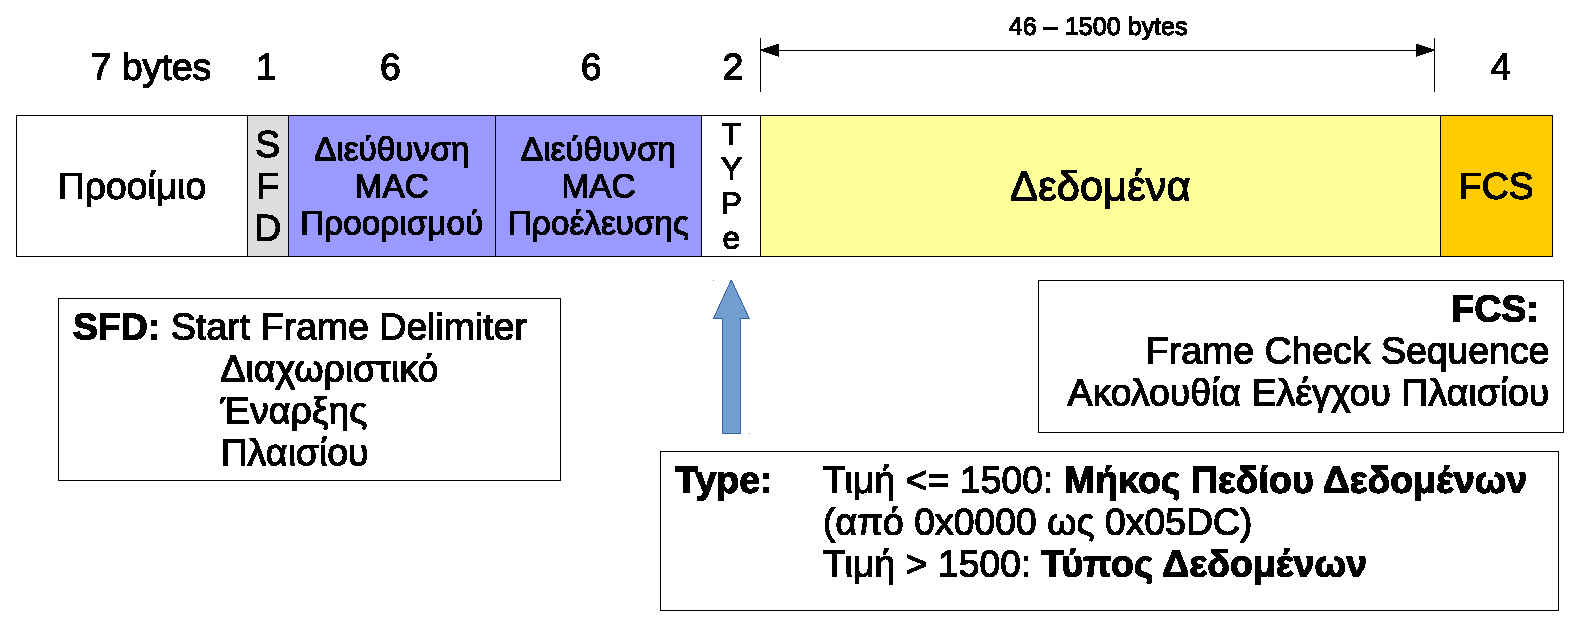
\includegraphics[width=0.95\textwidth]{images/chapter2/2-4}
  \caption {\textsl{Δομή Πλαισίου Ethernet}}
  \label{2-4}
\end{figure}

Μπορούμε να διακρίνουμε τα παρακάτω:

\begin{itemize}
\item Το \textbf{Προοίμιο} (Preamble). Για να συγχρονιστεί ο δέκτης με τον πομπό στέλνεται μια εναλλαγή ψηφίων 0 και 1 (αντιστοιχεί στον δεκαεξαδικό αριθμό 0x55, δείτε και τον πίνακα του δεκαεξαδικού παραπάνω). Στέλνονται επτά (7) τέτοιες οκτάδες. Στο τέλος στέλνεται μια οκτάδα 0xD5 που αποτέλει το σήμα για την έναρξη του πλαισίου και ονομάζεται \textbf{SFD} (Start Frame Delimiter). 
\item Ακολουθούν οι \textbf{Διευθύνσεις MAC Προορισμού και Προέλευσης} με κάθε μια να καταλαμβάνει χώρο 6 bytes.  Πρώτα μεταδίδεται η διεύθυνση προορισμού ώστε να ειδοποιηθεί έγκαιρα ο παραλήπτης και έπειτα μεταδίδεται η διεύθυνση του αποστολέα. 
\item Το πεδίο \textbf{Τύπος/Μήκος Δεδομένων} προσδιορίζει το είδος των δεδομένων που μεταφέρει το πλαίσιο ή πιο πρωτόκολλο ανώτερου επιπέδου τα έχει δημιουργήσει, αν η τιμή του είναι μεγαλύτερη από 1500. Αν η τιμή του είναι μικρότερη ή ίση με 1500 (0x5DC) τότε δηλώνει το μήκος των δεδομένων που μεταφέρει. To πεδίο έχει μήκος 2 bytes.
\item Ακολουθούν τα \textbf{Δεδομένα (Data)} τα οποία μπορεί να είναι από 46 ως 1500 οκτάδες.
\item Το πλαίσιο τελειώνει με το πεδίο \textbf{Ακολουθίας Ελέγχου Πλαισίου} ή FCS (Frame Check Sequence). Το πεδίο αυτό έχει μέγεθος 4 bytes και περιέχει πληροφορίες σύμφωνα με τις οποίες ο παραλήπτης μπορεί να ελέγξει αν το πλαίσιο έχει μεταδοθεί σωστά ή περιέχει σφάλματα. Για το σκοπό αυτό χρησιμοποιείται ο  αλγόριθμος \href{https://en.wikipedia.org/wiki/Cyclic_redundancy_check}{CRC32}.
\end{itemize}

Με το τέλος του πλαισίου ακολουθεί μια παύση μεγέθους 96 bit που ονομάζεται \emph{IPG ή InterPacket Gap} και είναι απαραίτητη προκειμένου τα κυκλώματα του δέκτη να επεξεργαστούν το προηγούμενο πλαίσιο και να ετοιμαστούν για τη λήψη του επόμενου.

Το μέγιστο μήκος ωφέλιμων δεδομένων ορίζεται από το πρότυπο ως 1500 bytes και ονομάζεται \emph{Μέγιστη Μονάδα Εκπομπής ή MTU (Maximum Transfer Unit)}. Η ελάχιστη ποσότητα δεδομένων που μπορεί να μεταφερθεί είναι 46 bytes. Μαζί με την επικεφαλίδα, το ελάχιστο επιτρεπτό μέγεθος πλαισίου είναι 64 οκτάδες (46 bytes δεδομένα και 18 επικεφαλίδα. Η επικεφαλίδα περιέχει τις δύο φυσικές διευθύνσεις (12 bytes), το πεδίο τύπος / μήκος δεδομένων (2 bytes) και το FCS (4 bytes)). Αν θέλουμε να στείλουμε μικρότερο πλαίσιο, τότε συμπληρώνουμε με μηδενικά (zero padding) ώστε να φτάσουμε το ελάχιστο μήκος.